\documentclass[12pt, a4paper]{article}

\usepackage[utf8]{inputenc}
\usepackage[T1]{fontenc}
\usepackage[russian]{babel}
\usepackage[oglav,spisok,boldsect,eqwhole,figwhole,hyperref,hyperprint,remarks,greekit]{./style/fn2kursstyle}
\graphicspath{{./style/}{./figures/}}
\usepackage{caption}
\usepackage{subcaption}

\usepackage{multirow}
\usepackage{supertabular}
\usepackage{multicol}



\usepackage{listings}
\usepackage{color}

\definecolor{dkgreen}{rgb}{0,0.6,0}
\definecolor{gray}{rgb}{0.5,0.5,0.5}
\definecolor{mauve}{rgb}{0.58,0,0.82}

\lstset{frame=tb,
	inputencoding=utf8,
	basicstyle=\ttfamily,
	extendedchars=\true,
	showspaces=\false,
	showstringspaces=\false,
	language=Python,
	aboveskip=3mm,
	belowskip=3mm,
	showstringspaces=false,
	columns=flexible,
	basicstyle={\small},
	numbers=left,
	numberstyle=\tiny\color{gray},
	keywordstyle=\color{red},
	commentstyle=\color{dkgreen},
	stringstyle=\color{mauve},
	breaklines=true,
	breakatwhitespace=true,
	tabsize=3
}











\title{Распознавание графиков решения \\ одномерного линейного уравнения переноса}
\author{О.\,Д.~Климов}
\supervisor{М.\,П.~Галанин}
\group{ФН2-61Б}
\date{2024}

\renewcommand{\labelenumi}{\theenumi)}
\begin{document}

\maketitle

\tableofcontents

\newpage

\section-{Введение}
Необходимость распознавания графика функций возникает в совершенно разных прикладных задачах науки и техники. Например, она непосредственно связана с проблемой восстановления графика решений уравнений по неточно заданным данных о решениях. В силу нелинейности распознавания изображений нахождение точных алгоритмов для такой задачи испытывало ряд трудностей. Однако с развитием программирования и вычислительной техники стало возможным решать данную задачу методами нейронных сетей.

\section{Постановка задачи}

\subsection{Формулировка}
Необходимо изучить методы численного решения линейного одномерного уравнения переноса. Составить и отладить программу для нахождения численного решения задачи Коши для указанного уравнения. Использовать шесть различных разностных схем:
\begin{enumerate}
	\item Явная схема с левой разностью на двух точках
	\item Явная схема с левой разностью на трех точках
	\item Неявная схема с левой разностью на двух точках
	\item Неявная схема с левой разностью на трех точках
	\item Схема Лакса
	\item Схема Лакса-Вендрофа
\end{enumerate}
Для всех схем использовать одинаковую систему тестов:
\begin{enumerate}
	\item Левый треугольник
	\item Правый треугольник
	\item Прямоугольник
	\item Синус
	\item "Зуб"
\end{enumerate}

Реализовать модель нейронной сети для распознавания решения на языке программирования Python. На основе модели разработать программу, которая по неточному решению возвращает более точное известное решение.

\subsection{Пример}
Основная задача работы состоит в том, чтобы создать программу, которая получала бы на вход неточное решение уравнения переноса и выдавала более точное соответствующее решение. На вход программы подается изображение с численным решением уравнения переноса, которое является неточным (рис.~\ref{image1}). Программа должна дать на выходе точное решение исходной задачи (рис.~\ref{image2}).

\begin{figure}[h]
	\begin{subfigure}[b]{0.5\textwidth}
		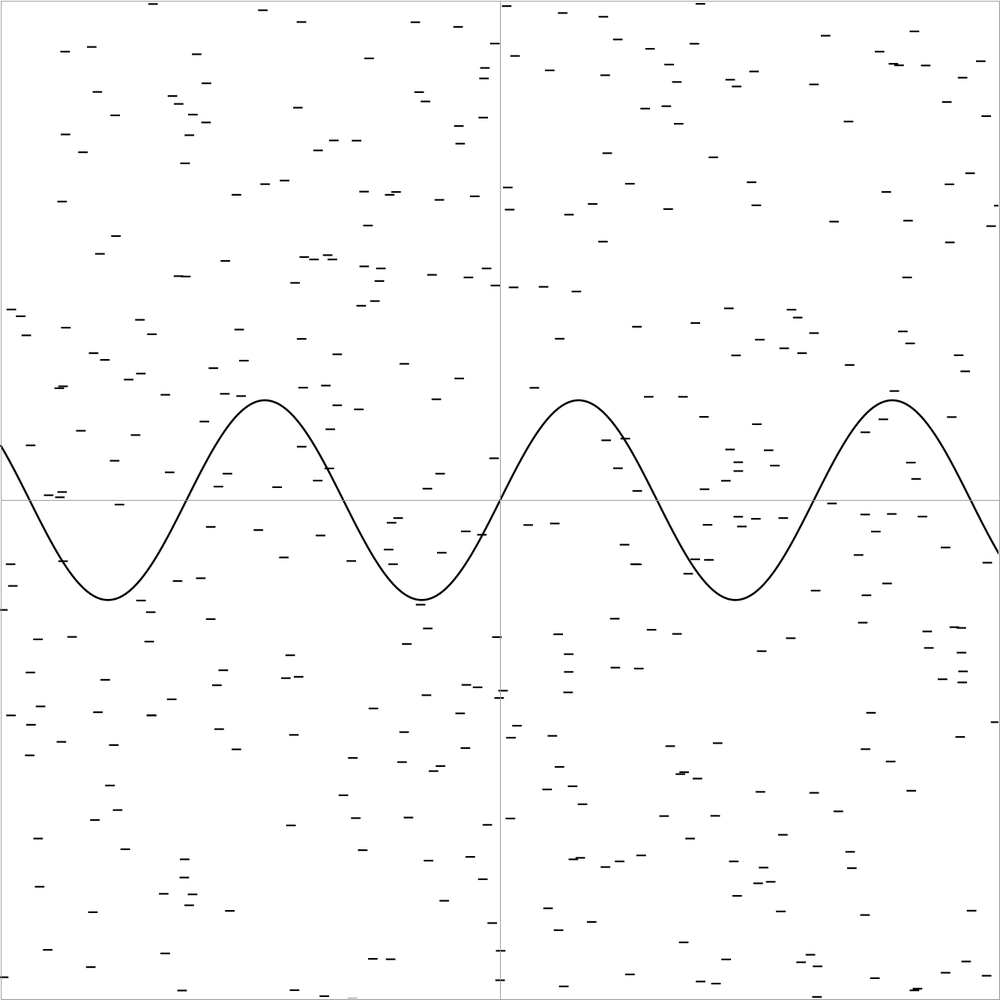
\includegraphics[width=\textwidth]{primer1_1}
		\caption{График неточного решения}
		\label{image1}
	\end{subfigure}
	\hfill
	\begin{subfigure}[b]{0.5\textwidth}
		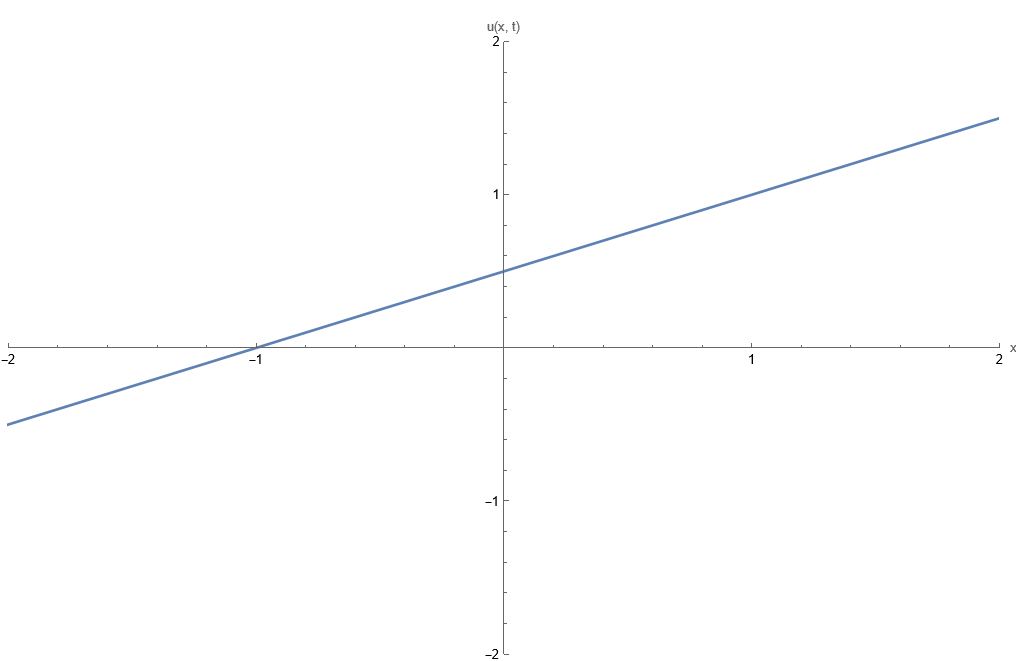
\includegraphics[width=\textwidth]{primer1_2}
		\caption{График точного решения}
		\label{image2}
	\end{subfigure}
	\caption{Иллюстрация задачи}
\end{figure}
\section{Задача Коши для линейного одномерного уравнения переноса}
Уравнение переноса является одним из фундаментальных уравнений математической физики, которое широко используется для описания движения сплошной среды. В то же время оно является простейшим представителем семейства гиперболических уравнений, которые определяются наличием действительных характеристик, число которых совпадает с числом неизвестных для системы уравнений первого порядка. Рассмотрим задачу Коши для уравнения переноса следующего вида:
\begin{equation}
	\begin{cases}
		\dfrac{\partial u}{\partial t} + \dfrac{\partial (a u)}{\partial x} = 0, \\
		u(x, 0) = u_0(x),
	\end{cases} 
	\text{где } u = u(x, t), \quad a = const > 0, \quad t \in (0, T), \quad x \in (-\infty, +\infty) .
\end{equation}


Приведем аналитическое решение. Уравнение можно записать в виде:
\begin{equation*}
	u_t + a u_x = 0
\end{equation*}
Запишем и решим характеристическое уравнение:
\begin{equation*}
	\dfrac{dt}{1} = \dfrac{dx}{a} = \dfrac{du}{0} \quad \implies  \quad 
	\begin{cases}
		u = C_1,\\
		x = a t + C_2
	\end{cases} 
	\quad \implies \quad
	\begin{cases}
		C_1 = u,\\
		C_2 = x - at
	\end{cases}
	 \quad \implies \quad
	 u = \psi(x-a t).
\end{equation*}
Применим граничные условия:
\begin{equation*}
	u(x, 0) = u_0(x),
	\quad \implies \quad
	\psi(x) = u_0(x),
	 \quad \implies \quad
	 u = u_0(x-a t).
\end{equation*}
Получим аналитическое решение уравнения $u = u_0(x-at)$. Решение заключается в сносе неизменного профиля по характеристикам. 

Важнейшим свойством рассматриваемого рещения будет являтся сохранение начального профиля: если начальное решение представляет собой, например, профиль буквы "М", то оно будет таким всегда.

\section{Численные методы решения задачи}
Целью построения методов численного решения данного уравнения является не собственно нахождения его решения, а исследование численного алгоритма на простейшем примере. Точное решение данного уравнения известно и тривиально. Однако в чрезвычайно большое количество математических моделей оператор переноса входит в качестве составной части. Это модели газодинамики, гидродинамики, переноса частиц и излучения, электродинамики и многие другие. Разработать для их численного решения численный метод можно только в том случае, если метод будет построен и успешно применен для данного простейшего уравнения, описывающего перенос.
\subsection{Описание методов}
Для численного решения задачи Коши для линейного одномерного уравнения переноса рассмотрим следующие схемы:



\begin{enumerate}
	
	\item \bf{Явная схема с левой разностью по двум точкам}:
	\begin{equation*}
		\widehat{y} = (1 - \gamma) y + \gamma y_{-1}.
	\end{equation*}
	
	\item \bf{Неявная схема с левой разностью по двум точкам}:
	\begin{equation*}
		\widehat{y} = \dfrac{\gamma}{1 + \gamma} \widehat{y}_{-1} + \dfrac{1}{1 + \gamma} y .
	\end{equation*}
	
	\item \bf{Явная схема с левой разностью по трем точкам}:
	\begin{equation*}
		\widehat{y} = (1 - \frac{3}{2}\gamma) y + \gamma(2y_{-1} - \frac{1}{2}y_{-2}) .
	\end{equation*}
	
	\item \bf{Неявная схема с левой разностью по трем точкам}:
	\begin{equation*}
		%\widehat{y} = (1 - \frac{3}{2}\gamma) y + \gamma(2y_{-1} - \frac{1}{2}y_{-2}).
		\widehat{y} = y - \frac{\gamma}{2} (-3y + 4y_{+1} - y_{+2})
	\end{equation*}
	
	\item \bf{Схема Лакса}:
	\begin{equation*}
		\widehat{y} = \dfrac{(y_{+1} + y_{-1}) - \gamma(y_{+1} - y_{-1})}{2} .
	\end{equation*}
	
	\item \bf{Схема Лакса-Вендрофа}:
	\begin{equation*}
		\widehat{y} = y - \gamma(F_p - F_l),
	\end{equation*}
	где $ F_p = \dfrac{(y_{+1} + y) - \gamma (y_{+1} - y)}{2}, \quad F_l = \dfrac{(y + y_{-1}) - \gamma (y - y_{-1})}{2} $.
\end{enumerate}

\subsection{Реализация}



\section{Метод улучшения решения с помощью нейронной сети}

Основной целью данной работы является создание программы, которая по известному точному решению сможет улучшить входное неточное. Для реализации такой программы был выбран метод, заключающийся в распознавании изображения нейронной сетью. Алгоритм заключается в следующем: нейронной сети, обученной на исключительно точных решениях, подается на вход неточное, которое она классифицирует. Как результат, нейронная сеть выдает метку соответствующего точного решения, которое и будет возвращать программа.

\subsection{Модель сверточной нейронной сети}

Сверточная нейронная сеть \cite{1} - модель нейронной сети, предложенная в 1988 году Яном Лекуном, которая и сегодня является одной из самых эффективных для распознавания образов на изображении. Структура сети однонаправленная и для обучения в большинстве случаев используется метод обратного распространения ошибки.

Основной особенностью сверточной нейронной сети является наличие комбинаций слоев свертки и пуллинга. Преимущества модели, заключается в способности улавливать пространственные взаимосвязи на изображении, что позволяет классифицировать одни и те же объекты независимо от их расположения и размера на изображении. Не менее значимым является меньшее количество настраиваемых весов, так как один набор фильтров как весы используется целиком для всего изображения, вместо того, чтобы создавать для каждого пикселя входного изображения свои коэффициенты как это делает перцептрон. Благодаря такой особенности, сверточная нейронная сеть требует меньшее количество времени для обучения. Также данная модель устойчива к повороту и сдвигу распознаваемого изображения. 

Для реализации своей модели выберем библиотеку $TensorFlow$ в силу ее простоты и полноты документации. Опишем основные шаги при создании модели сверточной нейросети с помощью библиотеки TensorFlow. 

 Модель нейросети представляет собой объект класса из TensorFlow, который мы назовем $Model$. При создании модели необходимо указать ее тип как $sequental$, что означает, что процесс вычислений будет последовательно идти по слоям. После создания модели необходимо добавить в нее слои, что можно сделать с помощью метода $.add$. Добавляя нужное нам количество уже встроенных в библиотеку слоев свертки $Conv2D$, указываем количество фильтров, их размерность и функцию активации. Добавляем слои пуллинга $MaxPooling2D$, указывая в параметрах слоя необходимую размерность подвыборки. Последними слоями будут полносвязные слои $Dense$, где мы указываем количество нейронов и также функцию активации. Количество вариантов ответа нейросети обозначим $output$. Наконец, соберем нашу модель с помощью метода $.compile$, в котором необходимо указать параметры функции оптимизатора, потерь и метрику обучения.  Для использования модели остается только ее скомпилировать с помощью метода $.compile$. 
 
 Библиотека позволяет сохранить параметры скомпилированной модели, что делает возможным встраивать уже созданный алгоритм распознавания в другие программы. Таким образом довольно практично можно создать свою модель нейронной сети для совершенно разных задач.
 
 \lstinputlisting[caption={Модель нейронной сети}, inputencoding=utf8]{code/Model.py}
 
 
\subsection{Распознавание решения}


\subsection{Результаты работы программы}


\section{Актуальность и перспективы задачи}
\section-{Заключение}
Таким образом в ходе работы были изучены численные методы решения уравнения переноса, проведено тестирование численных методов на 5 тестах, а также созданы несколько программ. Была создана программа, которая по неточному решения уравнения переноса возвращает точное. Была реализована программа на языке программирования С++17 для численного решения уравнения переноса различными схемами, а также реализованы 5 тестов. Реализована модель сверточной нейронной сети для распознавания решений уравнения на языке программирования Python 3.9 с помощью библиотеки машинного обучения TensorFlow 8.0. Изображения графиков решения создавались с помощью математического пакета Wolfram Mathematica 14. 

Как итог, реализована программа, которая с помощью модели сети улучшает неточное решение данного уравнения до точного.  



\clearpage
\begin{thebibliography}{1}

\bibitem{1} Галанин М.П., Савенков Е.Б. Методы численного анализа математических моделей. М.: Изд-во МГТУ им. Н.Э. Баумана. 2018. 592 с.


\bibitem{2} Tariq Rashid Make Your Own Neural Network // CreateSpace Independent Publishing Platform; 1st edition SAND96-0583 (March 31, 2016)


\bibitem{3} TensorFlow documentation. URL: https://www.tensorflow.org/?hl=ru (Дата обращения 17.01.2024)

%\bibitem{5} Keras documentation URL: https://keras.io (Дата обращения 17.01.2024)

%\bibitem{6} Гафаров Ф.М. Искусственные нейронные сети и приложения. г.Казань: Изд-во Казан. ун-та, 2018. –121 с


\end{thebibliography}

\end{document} 